\documentclass[a4paper,12pt]{report}

\usepackage[T1]{fontenc}
\usepackage[utf8]{inputenc}
\usepackage[english]{babel}

\usepackage[hidelinks]{hyperref}
\usepackage{graphicx}
\usepackage{caption}

\title{Connector - Reference manual }
\author{Gianluigi Forte}

\usepackage{listings}
\usepackage{color}

\definecolor{dkgreen}{rgb}{0,0.6,0}
\definecolor{gray}{rgb}{0.5,0.5,0.5}
\definecolor{mauve}{rgb}{0.58,0,0.82}

\definecolor{myBlue}{rgb}{0.33,0.57,0.79}
\definecolor{black!75}{rgb}{0.25,0.25,0.25}
\definecolor{purple}{rgb}{0.5,0.5,0.5}
\definecolor{OliveGreen}{rgb}{0.25,0.25,0.25}

\lstdefinelanguage{asymptote}{%
keywords=[1]{import, unitsize, add, shift,
 show, arc, include}, %pour asymptote + geometry
keywords=[2]{label, draw, dot, geometry, grid, triangleabc, perpendicularmark},% pour les autres extensions
keywords=[3]{pair, triangle, path}, % pour les classes
keywords=[4]{lightgray, black, gray, red}, %pour les couleurs
keywords=[5]{bp, pt, cm,  % unités
 N, E, S, W, NE, SE, SW, NW,
 NNE, ENE, ESE, SSE, SSW, WSW, WNW, NNW},% points cardinaux
comment=[l]{//},
otherkeywords={ -- , .. , :: , \^\^},
sensitive=true,
%morecomment=[s]{/*}{*/},
%string=[d]",
moredelim=*[s][\color{purple}]{"}{"},
moredelim=**[s][\color{OliveGreen}]{{$}{$}}
}


\lstset{%
language=asymptote,
keywordstyle=[1]\ttfamily\bfseries\color{myBlue},
keywordstyle=[2]\ttfamily\color{cyan},
keywordstyle=[3]\ttfamily\bfseries,
keywordstyle=[4]\ttfamily\color{Bittersweet},
keywordstyle=[5]\ttfamily\bfseries\color{brown},
identifierstyle=\ttfamily\color{black!75},
firstnumber=5
}% à compléter au besoin
%
%

\begin{document}
\maketitle

\section*{Introduction}

Connector is a library written in \emph{Asymptote} language to generate figures of electronic schematics. \LaTeX and \emph{Asymptote}, differently from other programs like Word or Write, are languages designed to produce documents with the best quality outputs for prints or presentations starting from a description, of the content to be produced, expressed programmatically in a source code text file and then produced in output after the compilation process. The idea behind the \emph{connector} library is to provide a ready to use set of functions written in Asymptote language to draw electrical components, link them with connection (wires), decorate with labels and produce the output figure as pdf or png files to be embedded in a larger Latex document or any kind of other usage like websites, videos, presentations and so on. 


\section*{Electronic Symbols}

Here a list of components to be used.
\begin{itemize}
\item node
\item resistor
\item capacitor
\item inductor
\item fuse
\item diode
\item relay
\item relay SPDT
\item IGBT
\item MOS
\item power ground
\item signal ground
\end{itemize}

In the folowing figures are shown the components, the anchor points with index number, and the origin position $(0,0)$ indicated with a red cross.

In figure \ref{nodeInfo} is shown a generic node.

\begin{figure}[h]
\centering
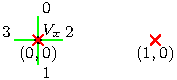
\includegraphics{nodeInfo}
\caption{Example of use of a generic node}
\label{nodeInfo} %Inserire sempre dopo caption
\end{figure}

To draw the component is possible to use the code:

\begin{lstlisting}
import connector;
import drawOptions;
import obj;
import resistor;

include 'common.asy';

Resistor r = Resistor((0,0), "$R_x$");
r.draw(DrawOption(
  showAnchor      = true,
  showAnchorLabel = true,
  showOrigin      = true));
\end{lstlisting}

\begin{figure}[h]
\centering
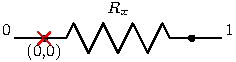
\includegraphics{resistorInfo}
\caption{Example of use of resistor}
\label{resistorInfo} %Inserire sempre dopo caption
\end{figure}

\begin{figure}[h]
\centering
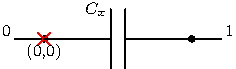
\includegraphics{capacitorInfo}
\caption{Example of use of capacitor}
\label{capaciorInfo} %Inserire sempre dopo caption
\end{figure}

\begin{figure}[h]
\centering
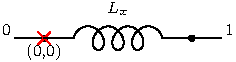
\includegraphics{inductorInfo}
\caption{Example of use of inductor}
\label{inductorInfo} %Inserire sempre dopo caption
\end{figure}

\begin{figure}[h]
\centering
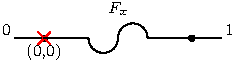
\includegraphics{fuseInfo}
\caption{Example of use of fuse}
\label{fuseInfo} %Inserire sempre dopo caption
\end{figure}

\begin{figure}[h]
\centering
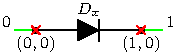
\includegraphics{diodeInfo}
\caption{Example of use of diode}
\label{diodeInfo} %Inserire sempre dopo caption
\end{figure}

\begin{figure}[h]
\centering
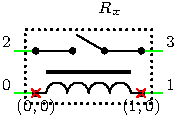
\includegraphics{relayInfo}
\caption{Example of use of relay}
\label{relayInfo} %Inserire sempre dopo caption
\end{figure}

\begin{figure}[h]
\centering
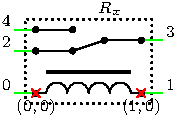
\includegraphics{relaySPDTInfo}
\caption{Example of use of relay SPDT}
\label{relaySPDTInfo} %Inserire sempre dopo caption
\end{figure}

\begin{figure}[h]
\centering
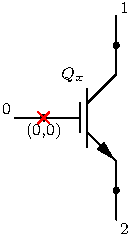
\includegraphics{igbtInfo}
\caption{Example of use of igbt}
\label{igbtrInfo} %Inserire sempre dopo caption
\end{figure}

\begin{figure}[h]
\centering
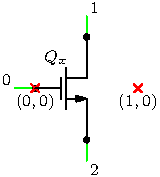
\includegraphics{mosInfo}
\caption{Example of use of MOS}
\label{mosInfo} %Inserire sempre dopo caption
\end{figure}

\begin{figure}[h]
\centering
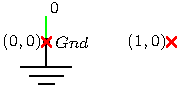
\includegraphics{gndPowerInfo}
\caption{Example of use of power ground symbol}
\label{gndPowerInfo} %Inserire sempre dopo caption
\end{figure}

\begin{figure}[h]
\centering
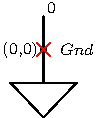
\includegraphics{gndSignalInfo}
\caption{Example of use of signal ground symbol}
\label{gndSignalInfo} %Inserire sempre dopo caption
\end{figure}

\end{document}